\begin{figure}[H]
\centering
\begin{annotatedFigure}
	{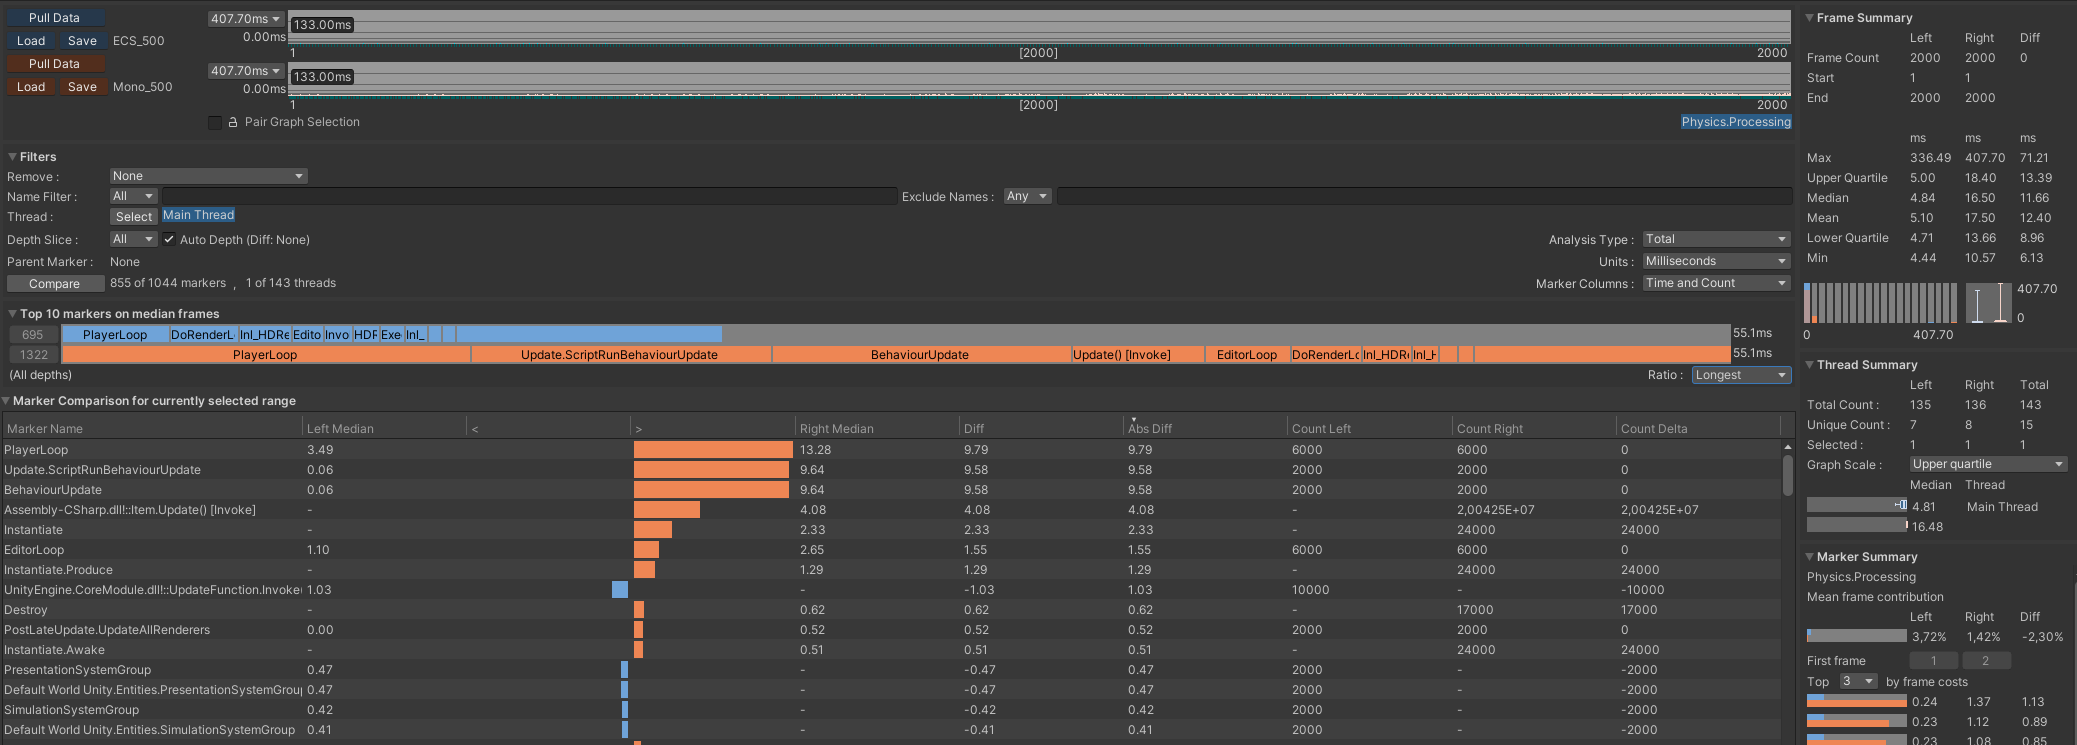
\includegraphics[scale=0.31]{Bilder/Profile Analyzer.png}}
	\annotatedFigureBox{-0.005,0.8046}{0.182,1.01}{A}{0.182,0.8046}
	\annotatedFigureBox{0.86,-0.01}{1.005,1.01}{D}{1.005,-0.01}
	\annotatedFigureBox{-0.005,0.4842}{0.857,0.5942}{B}{0.857,0.4842}
	\annotatedFigureBox{-0.005,-0.01}{0.445,0.4804}{C}{0.445,-0.01}
\end{annotatedFigure}
\caption{Der Profile Analyzer im Unity Editor. Es werden die Mono- und die ECS Messdaten des Spiels miteinander verglichen. Links oben (A) erkennt man welche Daten man gerade vergleicht und sieht dazu eine Timeline beider Daten. Die ECS Daten sind im Bild blau dargestellt, die Mono Daten rot. In der Mitte des Bildes (B) hat man den Vergleich des Median Bildes, also in diesem Fall des tausendsten Bildes von dem ECS und Mono. Deutlich zu erkennen ist die wesentlich kürzere Laufzeit des ECS Bildes. In dem unteren Teil (C) sieht man wichtige Spielfunktionen im Vergleich. Beispielsweise ist ganz oben der PlayerLoop (insgesamte Berechnungszeit eines Bildes). Dazu erkennt man an dem Balken, welcher der Spiele eine höhere Berechnungszeit hatte. Rechts (D) gibt es zusätzlich noch eine Zusammenfassung über die gesamte Anzahl an Bildern und Threads in beiden Spielen.}
\label{fig:profile_analyzer}
\end{figure}